\documentclass[12pt]{article}
\usepackage{titletoc}

\usepackage{sectsty}
\sectionfont{\fontsize{20}{18}\selectfont}
\subsectionfont{\fontsize{18}{18}\selectfont}
\subsubsectionfont{\fontsize{16}{18}\selectfont}

\usepackage{mathptmx}
\renewcommand*\rmdefault{mathptmx}




\usepackage{ucs}
\usepackage[utf8x]{inputenc} % Включаем поддержку UTF8
\usepackage[russian]{babel}  % Включаем пакет для поддержки русского языка

\usepackage[left=2cm, 		% Поле левое : 200 мм
			right=2cm, 		% Поле правое : 200 мм
			top=1cm,		% Поле верхнее: 100 мм
			bottom=2cm,		% Поле нижнее : 200 мм
			bindingoffset=0cm]{geometry}
			
\usepackage[pdftex]{graphicx, color}
\usepackage{color}
\usepackage{wrapfig}
\usepackage{float}
\usepackage{tikz}
 \usepackage{url}			% использование URL в библиографии
\usepackage{listings}		% использование листингов кода
\usepackage[nooneline]{caption} 
\captionsetup[table]{justification=raggedleft} 
\captionsetup[figure]{justification=centering,labelsep=endash}
\usepackage{array}

\usepackage{caption}
\usepackage{graphicx}


\renewcommand{\baselinestretch}{1.5}

% вставка листингов с кодом 
\lstset{inputencoding=utf8x, 		
		extendedchars=false, 
		keepspaces=true,
		language=c}

\renewcommand{\lstlistingname}{Листинг}
\usepackage[indentfirst,compact,topmarks,calcwidth,pagestyles]{titlesec}

%\usepackage{amsmath}
%\usepackage{mathtools}
\def\checkmark{\tikz\fill[scale=0.4](0,.35) -- (.25,0) -- (1,.7) -- (.25,.15) -- cycle;} 
\setcounter{tocdepth}{4} 	% chapter, section, subsection, subsubsection и paragraph
\setcounter{secnumdepth}{4}

\parindent=1,25cm				% красная строка = 1 см
\usepackage{enumitem}
\setlist[enumerate,1]{leftmargin=2.25cm}
\setlist[itemize]{leftmargin=2.25cm}
\graphicspath{{pics/}}
\DeclareGraphicsExtensions{{.jpg}}

\begin{document}
\fontsize{14}{16pt}\selectfont


	\begin{titlepage}
	
	\end{titlepage}

	
	\tableofcontents %Содержание
	\newpage
	
	
%====================================================================================
%Введение
%====================================================================================
	\part*{\centering Введение}
	\addcontentsline{toc}{part}{Введение}
	\hspace{\parindent}Имитационное моделирование —  метод, позволяющий строить модели, описывающие процессы так, как они проходили бы в действительности. Такую модель можно «проиграть» во времени как для одного испытания, так и заданного их множества. При этом результаты будут определяться случайным характером процессов. По этим данным можно получить достаточно устойчивую статистику.

А так же это метод исследования, при котором изучаемая система заменяется моделью, с достаточной точностью описывающей реальную систему, с которой проводятся эксперименты с целью получения информации об этой системе.
К имитационному моделированию прибегают, когда:

1. Дорого или невозможно экспериментировать на реальном объекте

2. Невозможно построить аналитическую модель: в системе есть время, причинные связи, последствие, нелинейности, стохастические (случайные) переменные

3. Необходимо сымитировать поведение системы во времени.


	Цель ИМ состоит в воспроизведении поведения исследуемой системы на основе результатов анализа наиболее существенных взаимосвязей между её элементами или другими словами — разработке симулятора (англ. simulation modeling) исследуемой предметной области для проведения различных экспериментов.

В рамках данного курсового проекта разрабатывается имитационная модель пересадочного узла станции Московского метрополитена Третьяковская. Данный узел обеспечивает ежедневно перемещение более 70 тысяч людей. В часы наиболее плотного пасажиропотока в некоторых участках станции образуется давка. Целью данного курсового проекта является анализ и выявление узких мест транспортного узла а так же выработка предложений для улучшения ситуации. 

%====================================================================================	
	\newpage
	\section{Предпроектное иследование}
		\subsection{Основные положения среды моделирования AnyLogic }
			\hspace{\parindent} 
Для написанная модели было выбрано программное обеспечение для имитационного моделирования AnyLogic. В AnyLogic реализованны виды ИМ. А именно: 


\begin{itemize}
	\item Многоподходное моделирование
	\item Агентное моделирование
	\item Системная динамика
	\item Дискретно-событийное моделирование
	\item Моделирование динамических систем

\end{itemize}
\indent Для реализации модели пассажиропотоков наиболее подходящим является подход моделирование динамических систем. Он по сути является прародителем системно-динамического подхода моделирования. Моделирование с помощью данного подхода используется в мехатронике, электрической, химической и других инженерных областях в качестве стандартного этапа процесса разработки. С математической точки зрения динамическая система представляет собой набор переменных состояния и алгебраических дифференциальных уравнений различного вида, заданных для этих переменных и описывающих их изменение с течением времени. В отличие от системной динамики, переменные здесь несут некоторый "физический" смысл: координаты местоположения, скорость, ускорение, сила, концентрация и.т.д., они, как это следует из их смысла, непрерывны и не являются агрегированными величинами, отражающими, например, общее количество или среднее значение нескольких сущностей. [3]\\
\newpage
		\subsection {Пешеходная библиотека среды моделирования AnyLogic }
			\hspace{\parindent}
			
 \begin{wrapfigure}{r}{0.5\textwidth}
  	\begin{center}
  	  	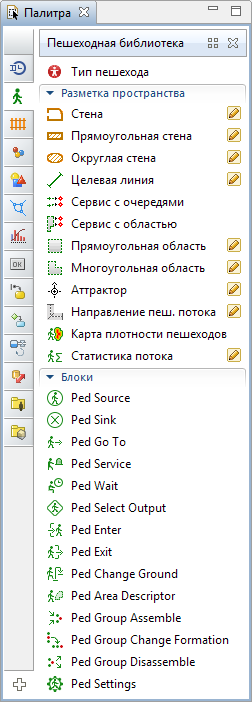
\includegraphics[width=0.3\textwidth]{ped_lib.png}
 	 \end{center}
	  	\caption{Элементы пешеходной библиотеки}
\end{wrapfigure}

Для моделирования пасажиропотоков была выбрана Пешеходная библиотека AnyLogic.Она является высокоуровневой библиотекой моделирования движения пешеходов в физическом пространстве. Она позволяет моделировать здания, в которых движутся пешеходы (станции метро, стадионы, музеи), а также улицы и другие места большого скопления людей. С помощью Пешеходной библиотеки легко можно собирать статистику, эффективно визуализировать моделируемый процесс для валидации и представления модели. Можно собирать статистику плотности пешеходов в различных областях модели для того, чтобы убедиться, что сервисы смогут справиться с потенциальным ростом нагрузки, вычислить время пребывания пешеходов в каких-то определенных участках модели, выявить возможные проблемы, которые могут возникнуть при перепланировке интерьера здания, и т.д. В моделях, созданных с помощью объектов Пешеходной библиотеки, пешеходы движутся в непрерывном пространстве, реагируя на различные виды препятствий в виде стен, различных областей и других пешеходов. 

 Модели движения пешеходов состоят из двух составляющих – среды и поведения. Под средой подразумеваются объекты физической среды - стены, различные области, сервисы, очереди и т.д. Объект среды задается специальным графическим элементом разметки, у которого задаются параметры объекта среды. Ресурсы (сервисы) также являются объектами среды. Поведение пешеходов задается блок-схемой. 

 Основным объектом библиотеки является пешеход. Пешеход задается с помощью объекта типа Ped. Пешеход “обитает” в заданном физическом пространстве (моделируемой среде) и передвигается согласно заданным правилам. С другой стороны, тип пешехода унаследован от типа агента Agent, поэтому пешеходы перемещаются по блок-схеме так же, как агенты. 

 Пешеходная библиотека совместима с Библиотекой моделирования процессов AnyLogic. Это позволяет использовать в пешеходных моделях любые объекты Библиотеки моделирования процессов, делая возможным создание сложных моделей, состоящих из блок-схем Библиотеки моделирования процессов и среды Пешеходной библиотеки. Такая совместимость возможна благодаря наличию в Пешеходной библиотеке объектов, превращающих агентов в пешеходов и наоборот. 

 Блок-схемы пешеходных моделей строятся с помощью объектов, содержащихся в Пешеходной библиотеке. Тип агента Ped является базовым типом для моделирования пешеходов. Как всегда, в библиотеке есть объекты для создания пешеходов и управления потоком пешеходов. 

Пешеходы создаются объектами PedSource, затем они могут быть добавлены в моделируемую среду и направлены далее согласно созданной диаграмме процесса, составленной из блоков Пешеходной библиотеки. Хотя пешеходы движутся в блок-схеме, их движение между блоками блок-схемы определяется моделируемой средой. Например, продолжительность пребывания в объекте PedGoTo зависит от скорости пешехода, плотности[3] пешеходов в данной области и других параметров среды.

\newpage
		\subsection {Железнодорожная библиотека среды моделирования AnyLogic }
			\hspace{\parindent}
			
 \begin{wrapfigure}{r}{0.5\textwidth}
  	\begin{center}
  	  	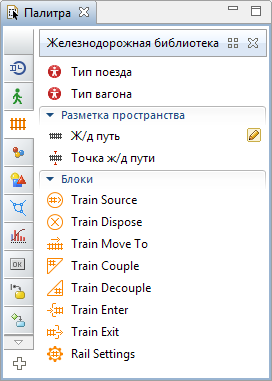
\includegraphics[width=0.3\textwidth]{rail_lib.png}
 	 \end{center}
	  	\caption{Элементы железнодорожной библиотеки}
\end{wrapfigure}
При описаниии логики железнодорожного транспорта использовалась железнодорожная библиотека AnyLogic.Она  поддерживает детализированное моделирование высокой точности (индивидуальные размеры вагонов, точная топология путей и стрелок, ускорение и торможение поездов), но это моделирование имеет высокую динамику в исполнении, что может быть важно при оптимизации в поисках лучшей стратегии.

Двумя основными входными составляющими железнодорожной модели являются топология железнодорожной сети и операционная логика железнодорожного узла.

Топология железнодорожного узла (это может быть сортировочная станция, пути погрузки/разгрузки и т.д.) состоит из специальных элементов разметки пространства, разработанных для моделей железной дороги: путей, стрелок и элементов, задающих смещение на пути (точка ж/д пути). Можно как нарисовать эти фигуры вручную в графическом редакторе, так и создать их программно, например, считав данные из базы данных.

Железнодорожная библиотека поддерживает очень простой высокоуровневый интерфейс задания операций железнодорожного узла. Библиотека содержит семь объектов:

\begin{itemize}
	\item TrainSource 
	\item TrainDispose
	\item TrainMoveTo
	\item TrainCouple 
	\item TrainDecouple
	\item TrainEnter 
	\item TrainExit
\end{itemize}

С помощью этих объектов можно выполнять любые операции с поездами и вагонами без необходимости писать программный код. Более того, диаграммы процессов железнодорожного узла могут включать в себя объекты Библиотеки моделирования процессов, такие, как Delay, SelectOutput, Hold, Seize, Release, Queue, и т.д. Это означает, что теперь операционная логика железнодорожных узлов может быть полностью задана графически простым перетаскиванием объектов (в стиле drag-and-drop).[3]


\newpage
\section{Техническое задание}
	\subsection{Введение }
Программный продукт компании  The AnyLogic Company AnyLogic является мошным инструментом ИМ. Инструмент обладает современным графическим интерфейсом и позволяет использовать язык Java для разработки моделей.Среда моделирования AnyLogic поддерживает проектирование, разработку, документирование модели, выполнение компьютерных экспериментов с моделью, включая различные виды анализа — от анализа чувствительности до оптимизации параметров модели относительно некоторого критерия. Все вышеперечисленные приемущества позволяют выбрать эту среду для разработки модели.
	
	
	\subsection{Общие сведения }
	
	Основание для разработки: задание на курсовой проект.
	
	Заказчик: Кафедра «Компьютерные системы автоматизации производства» МГТУ им. Н.Э.Баумана
	
	Разработчик: студент кафедры «Компьютерные системы автоматизации производства»  Айбушев Т.К.
	
	Наименование темы разработки: «Моделирование транспортного узла станции метро Третьяковская»
	
	\subsection{Назначение разработки }
	Анализ и выявление узких мест транспортного узла, выработка предложений для улучшени ситуации.
	\subsection{Требования к модели }
		\subsubsection{Требования к порядку сбора статистический данных }
		Статистические данные деобходимо собирать непосредственно на станции в момент наибольшей нагрузки станции а именно в промежуток времени с 9:00 до 10:00 в будний день. Для синхронизации собранных данных необходимо производить сбор данных в одно время со всех направлений пасажиропотоков.  А именно по одному статисту для каждого из направлений. 
		\subsubsection{Требования к модели}
\begin{itemize}
	\item Необходимо смоделировать часть всего пересадочного узла, а именно ту часть куда приходят поезда от станции Новокосино. 
	\item Моделирование производить в среде AnyLogic
	\item Статистику оформлять в унифицированном виде.
	\item Выработать предложения по улучшению станции
\end{itemize}

		\subsubsection{ Требования к статистическим данным }
		Данные должны соответсвовать реальному положению на станции в момент сбора статистики. 
		\subsubsection{Требования к результатам моделирования}
		Модель должна в полной мере соответствовать статистическим данным собранным на станции. Необходимо удостоверится в их соответствии.  
		\subsubsection{Требования к составу и параметрам технических средств}
		Модель должена работать на компьютерах со следующими
характеристиками:
\begin{itemize}
	\item Объем ОЗУ не менее 2048 Мб;
	\item 500MB свободного дискового пространства;
	\item Cовременный процессор для хорошей производительности.;
	\item Рекомендуется использовать мышь;

\end{itemize}

		\subsubsection{Требования к маркировке и упаковке }
Требования к маркировке и упаковке не предъявляются
		\subsubsection{Требования к составу и параметрам технических средств}

Система должна работать под управлением следующих ОС: Windows 7
Для моделированиия необходимо использовать программный продукт компании  The AnyLogic Company AnyLogic
		\subsubsection{Требования к транспортированию и хранению }
Требования к транспортированию и хранению не предъявляются.
		\subsubsection{Требования к транспортированию и хранению}
		Требования к транспортированию и хранению не предъявляются.
				\subsection{Стадии и этапы разработки }
Плановый срок начала разработки – 01 сентября 2014г.
Плановый срок окончания разработки – 22 декабря 2014г.
Этапы разработки:
\begin{itemize}
	\item Концептуальный этап проектирования системы;
	\item Технический этап проектирования системы;
	\item Рабочий этап проектирования системы.
\end{itemize}
	\subsection{Порядок контроля и приемки}
	Прием и контроль работоспособности осуществляется научным руководителем, после полного согласия разработчика о работоспособности и соответсвии действительности модели. 

\newpage

\section{Концептуальный этап проектирования системы}
		\subsection{Выделение ключевых элементов моделирования}
 \begin{wrapfigure}{r}{0.5\textwidth}
  	\begin{center}
  	  	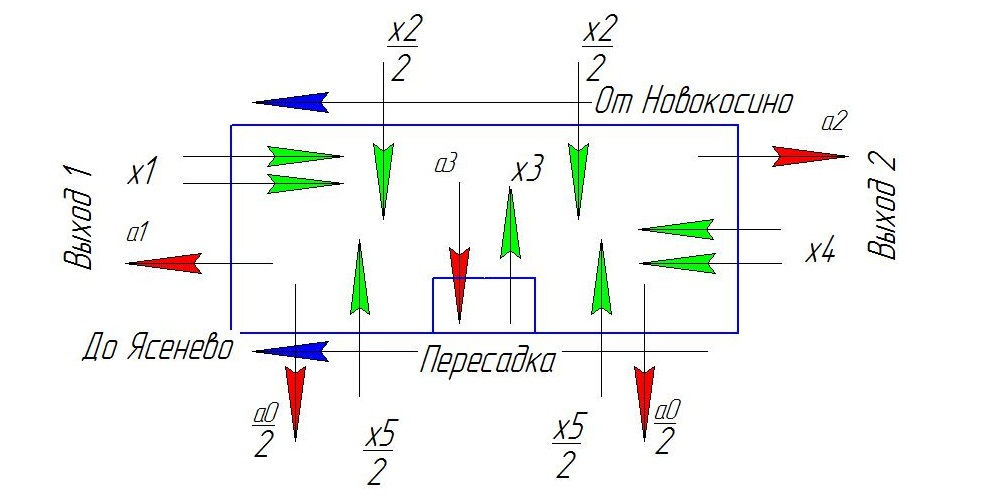
\includegraphics[width=0.6\textwidth]{shema.jpg}
 	 \end{center}
	  	\caption{Схема пасажиропотоков}
\end{wrapfigure}	


		Для полного описания модели необходимо составить схему пассажиропотоков. На станции есть два выхода, одна пересадка и одна кроссплатформенная пересадка. Соответственно из каждого и направлений пешеходы могут как уходить так и приходить.  Исключения составляют только поезда от станции Новокосино. Так как Третяковская является для них конечной они не могут попасть в поезд.
 \begin{wrapfigure}{r}{0.5\textwidth}
  	\begin{center}
  	  	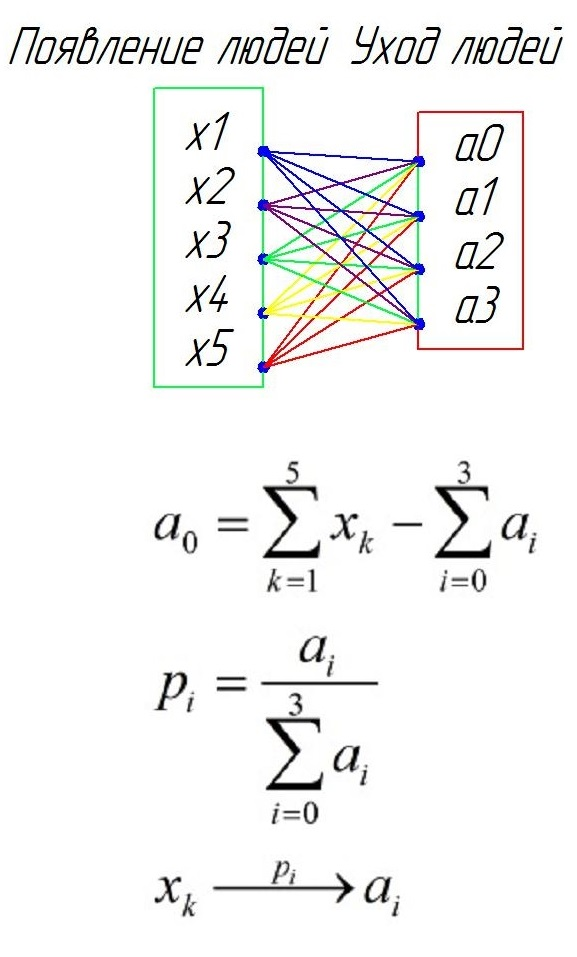
\includegraphics[width=0.3\textwidth]{enter_exit.jpg}
 	 \end{center}
	  	\caption{Взяимосвязь выходов и  входов}
\end{wrapfigure}
  
		Наиболее затрудненное место для сбора статистики является определение количества людей делающих кроссплатформенную пересадку. Поэтому количество людей соверщажщих такую пересадку мы примем неизвестной. Соответственно для каждого из потоков необходисо собрать статистику, а оставшийся переход вычеслить как единственный неизвестный.
		
		  Пешеходы с вероятность pi  попадают в каждый выход.  Вероятности для каждого из направления необходимо вычеслить.

		\subsection{Выделение ролей в разработке проекта }
		
Если формально распределить обязанности каждого из этапов моделирования, то можно выделить 5 основных ролей:		
	\begin{itemize}
		\item Аналитик;
		\item Статист;
		\item Методист;
		\item Разработчик;
		\item Концептуальный проектировщик ;
	\end{itemize}	
	
		\subsection{Распределение автивностей каждой роли}

Статист занимается сбором статитики и переводом статистики в унифицированный вид. 

Методист занимается определением ключевых параметров и определением принципов сбора данных. Он непосредственно взаимодействует со статистом, формулируя методику сбора данных.

Аналитик определяет механизм сбора данных, а так же анализирует собранную статистику. Аналитик вместе с разработчиком занимается адаптацией модели т.е. соотносит реальные статистические данные со статистикой собранной в модели.

Разработчик внедряет собранные статистом данные в модель. Формирует данные расписания прибытия поездов, пассажиропотоков, направлений движения и тд. в подходяший для системы вид, а так же непосредственно реализует логику системы сформулированную концептуальным проектровщиком.

 Концептуальный проектировщик озабочем наиболее фундаментальными вопросами системы. Непосредственно он выделяет необходимые элементы для моделирования.  Формирует логическую схему системы в общем виде и структурирует модель выделяя структурные общности.[2]




\newpage
\section{Технический этап проектирования системы}
		\subsection{Создание схемы пассажиропотоков}

	
Первым этапом технического проектирования пассажиропотоков является создание  схемы пассажиропотоков. На этом этапе только моделируются направления вдижения пешеходов которые на этапе концептуального проетиролвания были выбраны как наиболее значимые. Схемы движения пассажиропотоков изображены  листе 2.  И в соотвествие с ним формируется и реальная логика системы.

 \begin{wrapfigure}{r}{0.7\textwidth}
  	\begin{center}
  	  	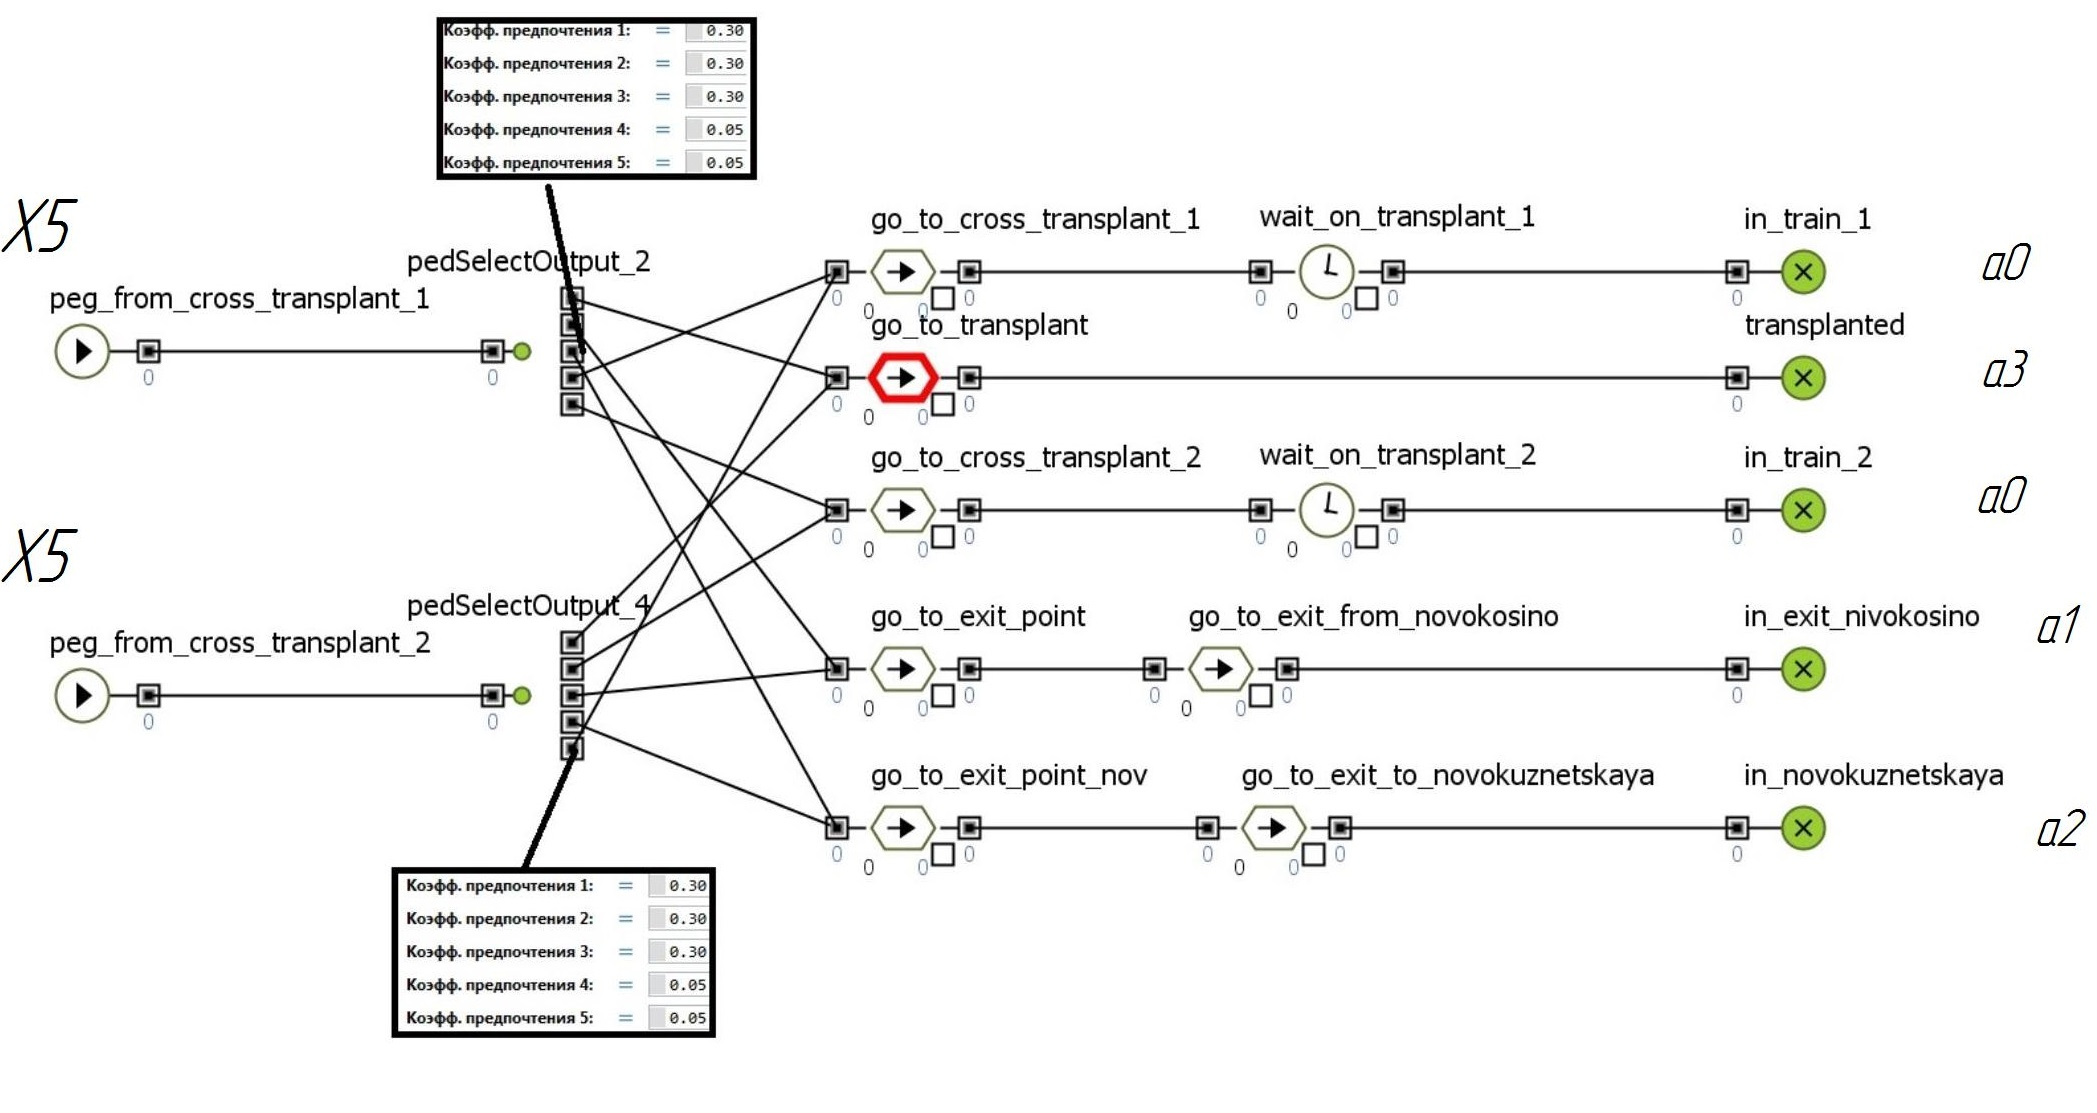
\includegraphics[width=0.8\textwidth]{logic_1.jpg}
 	 \end{center}
	  	\caption{Пример реализации логики}
\end{wrapfigure}

  В рамках данное задачи было принято решение реальзовывать модель в плоском виде, без использования трехмерной графики. Это в свою очередь накладывает некоторые ограничения на реализацию системы. Этот конфликт возникает когда необходимо учитовать перемещение пешеходов по высоте. Так при переходе и пересадке пешеходы находятся на разных уровнях. Поэтому этот элемент доступен только для пешеходов соверш	ающрих переход. 

Еще интересен момент перемещения пешеходов на экскалаторе. Использование стандартных элементов обслуживания мешеходов в данной проблеме не возможно. Так как обслуживание подразумевает неподвижность обслуживаемых объектов. В таком сличае был применен другой прием. В момент когда пешеходы попадают на эскалатор их скорость снижается до скорости движения экскалатора, что и моделирует относительное перемещение пешеходов. 

Еще одним ограничением выступило количество элементов которые можно использовать в пешеходной библиотеке в университетской лицензии AnyLogic. Поэтому, например, количество мест откуда появляются пешеходы из вогона было минимизированного до одного. При этом все пешеходы появляются в одном месте равно распредленно по длине линии появления. А так же это позволило смоделировать только один участок узла из трех. Но всвязи с тем, что маштабирование моделей такого типа задача достаточно простая, это не уменшает сложность написания модели.  [1]
   
		\subsection{Создание схемы движения поездов}
Для описания поездов использовалась железнодорожная библиотека. После въезда поезда на станцию он останавливается, некоторое время ждет потом отправляется. Все эти действия были описаны в модели. 
 \begin{wrapfigure}{r}{0.7\textwidth}
  	\begin{center}
  	  	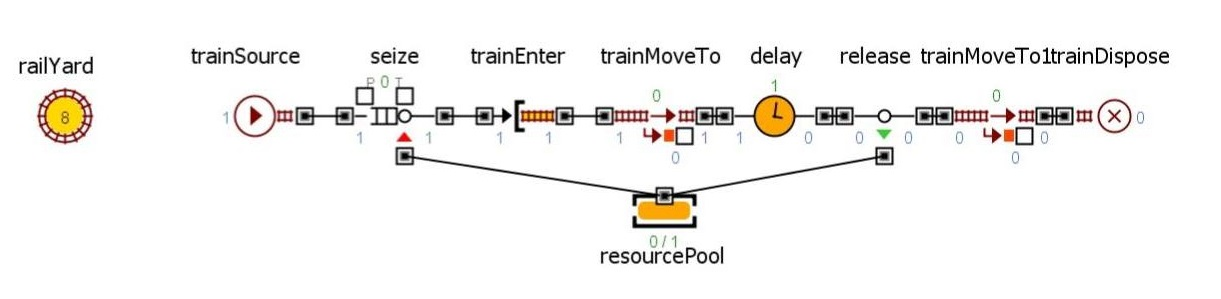
\includegraphics[width=0.8\textwidth]{train.jpg}
 	 \end{center}
	  	\caption{Пример реализации логики движения поездов}
\end{wrapfigure}

Описание элементов схемы(см. Рис. 6 ). Объект RailYard задает сеть железнодорожных путей и стрелок, основываясь на заданной группе фигур, проверяет правильность сети и визуализирует работу узла с помощью анимации во время выполнения модели. Этот объект необходим для любой железнодорожной модели. Объекта TrainSource создает поезда, помещает их на один из путей ж/д узла, и вставляет заявку типа Train в диаграмму процесса поезда. Объект Seize захватывает заданное количество ресурсов. Release освобождает заданное количество ресурсов, заданных указанным объектом ResourcePool. ResourcePool задает набор ресурсов, которые могут захватываться и освобождаться заявками с помощью объектов Seize, Release и Service TrainEnter помещает поступающую в объект заявку-поезд на заданный путь железнодорожной сети. TrainExit извлекает поступающий в объект поезд из железнодорожной сети и передает заявку-поезд далее. TrainMoveTo единственный объект, который управляет движением поезда. Поезд может перемещаться только тогда, когда он находится в объекте. [3]

		\subsection{Внедрение статистики}
		
 \begin{wrapfigure}{r}{0.7\textwidth}
  	\begin{center}
  	  	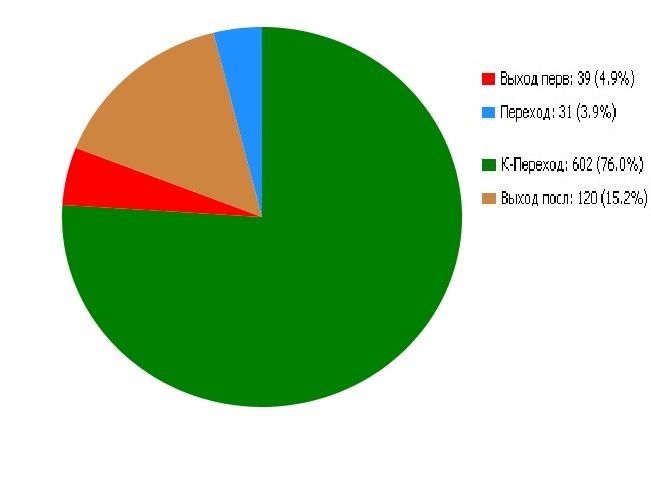
\includegraphics[width=0.4\textwidth]{stat_raspr.jpg}
 	 \end{center}
	  	\caption{Пример распределения потоков для выходо из поездов от Новокосино}
\end{wrapfigure}
Объект сбора статистики Статистика вычисляет основную статистическую информацию (среднее значение, минимум, максимум и т.д.) для последовательности измеренных значений (типа double).Для внедрения статистики ее предварительно необходимо было переработать. И вычислить распределения пассажиров по направлениям. На Рис. 7 приведен пример распределения для  выходо из поездов от Новокосино. Статитистика по всем направления в Приложении. Имея статистические данные их можно внедрять в модель. Для этого использовался объект pedSelectOutput он направляет входящих в объект пешеходов на один из пяти выходных портов. Условия вычисляются последовательно: вначале проверяется условие, заданное для первого порта (Условие 1). Если оно выполняется, то пешеход покидает объект через первый (самый верхний) порт out1. Если нет, то проверяется следующее условие, в случае выполнения которого пешеход покинет объект через порт out2, и так далее, если ни одно из четырех условий выполнено не будет, то будет выбран последний порт out5. Условиями в нашем случае выступали коэффициенты предпочтения.



		\subsection{Создание раписания}
		
 \begin{wrapfigure}{r}{0.7\textwidth}
  	\begin{center}
  	  	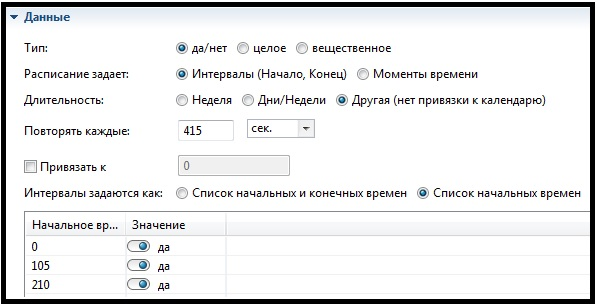
\includegraphics[width=0.6\textwidth]{sch.jpg}
 	 \end{center}
	  	\caption{Расписание}
\end{wrapfigure}

Важный этап этап моделирования это непосредственно внедрение собранной стастики в модель. Расписание может работать в одном из двух режимов: задание интервалов времени или задание моментов времени.

Первый режим (интервалы) обычно используется для задания того, как значение какой-то величины непрерывно меняется во времени (обычно - с определенной цикличностью). В данном случае в любой момент времени задаваемая расписанием величина будет иметь какое-то значение. С помощью интервалов задаются и расписания работы смен рабочих, и изменение интенсивности создания заявок или пешеходов, и многое другое.

Второй (моменты времени) используется тогда, когда задается последовательность ключевых моментов, которым соответствуют заданные для них значения. Как и было реализовано расписание прибытия поездов: в моменты прибытия в пешеходной модели железнодорожного вокзала на перроне появляется заданное расписанием количество пассажиров. 
		\subsection{Связывание прибытия поездов с пассажиропотоками}
Для этого использовалось действия при входе в объект delay. Когда поезд отстанавливается на станции, сразу же выходят пешеходы. 		
\newpage
\section{Рабочий этап проектирования системы}
		\subsection{Сбор статистики на станции}
		
		Сбор статистики происходил в утром 17 ноября 2014 года. Для сбора статистика понадобилось пять статистов. Каждый из статистов собирал информацию, по каждому из напрвлений. Время фиксировалось по факту прибытия поезда.  Нас интересовало сколько людей успевают проти к тому или иному направлению за промежутки между прибытия поездов. В некоторых напрвления как выходы из станции, возле экскалаторов скапливалось много людей, количество людей стоящих в очереди оченивалось примерно 4-6 человек на квадратный метр.
		
 \begin{wrapfigure}{r}{0.7\textwidth}
  	\begin{center}
  	  	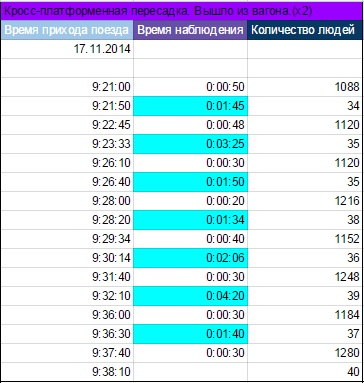
\includegraphics[width=0.6\textwidth]{stat_example.jpg}
 	 \end{center}
	  	\caption{Пример оформления статистики}
\end{wrapfigure}
На Рис. 8 приведен пример статистики для кроссплатформенной станции. В тот виде в котором она представлена на картинке это уже конечный вариант. Тут уже просчитаны промежутки времени между прибытиями поездов.		 
		   Наиболее сложный для сбора статистики участок был - выход пассажиров из вагона от станции метро Новокосино, т.к. для них это конечная станция и весь вагон выходит одновременно. Как не странно это достаточно большой поток людей. Для упрошения подсчетов было принято решение собирать стастику из каждого выхода из вагона, т.е. кажлый следующий приезд поезда означал смену выхода для сбора статистики.  Так пройдя большую часть выходов из вагонов было собранно достаточно статистики по каждому из вагонов и было построенно распределение количества пассажиров выходящих из вагонов. 
		\subsection{Сбор статистики с модели}
		
 \begin{wrapfigure}{r}{0.7\textwidth}
  	\begin{center}
  	  	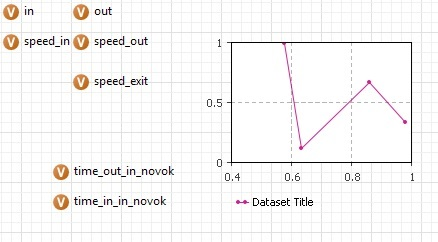
\includegraphics[width=0.6\textwidth]{stat_any_logic.jpg}
 	 \end{center}
	  	\caption{Пример сбора статистики в AnyLogic}
\end{wrapfigure}		
		
Для проверки адекватности модели было необходимо проверить соответствует ли статистика собранная на станции модельной статистике. Для этого использовались инструмены для сбора статистики AnyLogic. Объект сбора статистики Статистика вычисляет основную статистическую информацию (среднее значение, минимум, максимум и т.д.) для последовательности измеренных значений (типа double). Так на Рис.10 показан пример элементов необходимых для сбора статистики. Так например in и out это переменные, они помогают отсеживать изменения значания, в данном случае, времени прихода обекта типа Ped в заданную область.
\subsection{Анализ проблемным мест модели}

		
		
После проверки адекватности модели для определения узких мест использовалась карта плотности. На ней можно проследить в каких местах наиболее плотный пасажиропоток.

 \begin{wrapfigure}{r}{0.7\textwidth}
  	\begin{center}
  	  	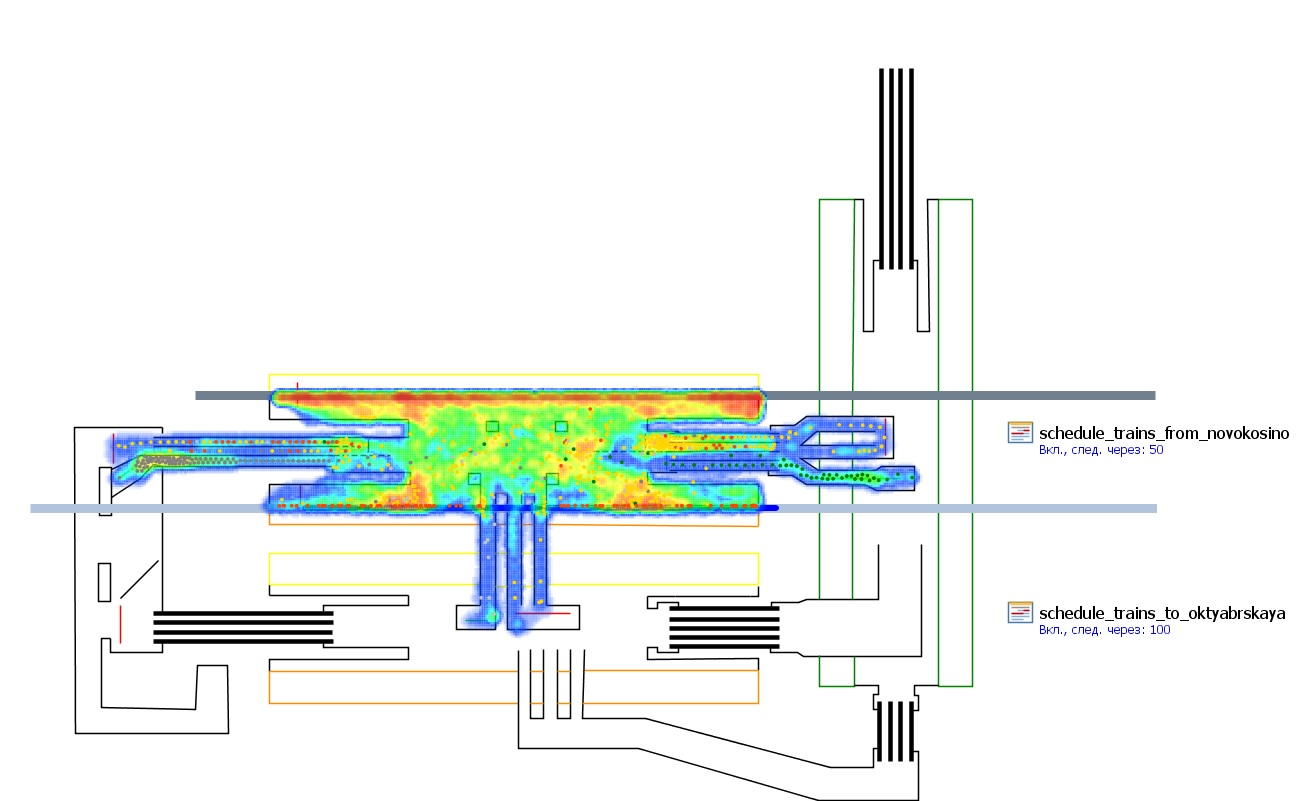
\includegraphics[width=0.4\textwidth]{den_map.jpg}
 	 \end{center}
	  	\caption{Карта плотности подели}
\end{wrapfigure}	

   В нашем случае осложнены выходы с пирона на станцию они подствечивается красных цветом на карте плотности. А так же выход со станции в направлении станции Новокузнетская. Для более точного определения плотности пассажиропотоков использовался метод getCurrentDensity, который позволяет вычеслить точное значение плотности для конкретной точки. Конкретные значения представлены на листе 6. 		
		\subsection{Внедрение изменени в модель}

\begin{wrapfigure}{r}{0.7\textwidth}
  	\begin{center}
  	  	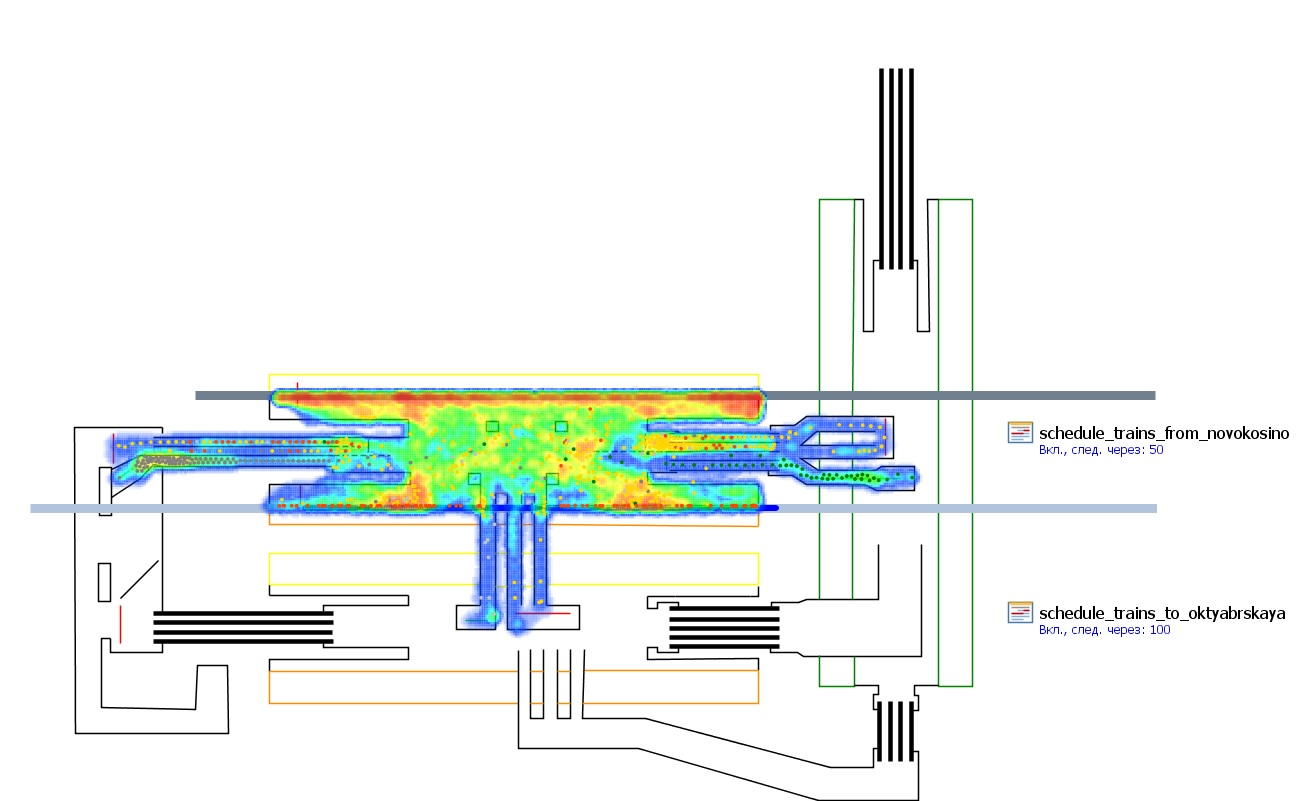
\includegraphics[width=0.4\textwidth]{den_map_new.jpg}
 	 \end{center}
	  	\caption{Карта плотности подели}
\end{wrapfigure}		

		По Рис.12 видно, что больше всего людей скуапливается у выходов на станцию с платформы. Как один из вариантов решения такой проблемы было предложено применить изменение геометрии станции. Новая карта плотности показывает, что если снести некоторые стены на станции и обновить экскалаторы, то большая часть проблем с давной будет решена.Во  время иследования модели были расмотрены и друге варианты. Разного рода вариации геомметрии стен и многое другие. Так как станция далеко не новая,  проектировалась для совсем другой нагрузки, то такая реконструкция  уже необходима и достаточно не сильно финансозатратна. 
		


			%====================================================================================
	

%====================================================================================
	%Список Литературы	%====================================================================================
\part*{\centering Список литературы}
\addcontentsline{toc}{part}{Список литературы}

	\bibliographystyle{plain}		
	\bibliography{biblio}
\hspace{\parindent} \hspace{\parindent}


1) Кельтон В., Лоу А. Имитационное моделирование 3-е изд. - СПб: Питер, 2004. -847 

2) Прицкер, А. Алан Б. Введение в имитационное моделирование и язык СЛАМ II  Москва : Мир, 1987 . – 644 с. 

3) www.anylogic.ru/anylogic/help/

	\newpage	%====================================================================================	
	%Приложения
	\definecolor{white}{rgb}{1,1,1}
	\lstset{backgroundcolor=\color{white}, basicstyle=\footnotesize, tabsize=4, frame=none}		%====================================================================================
	\part*{Приложение}
	\addcontentsline{toc}{part}{Приложение A. }
		\begin{lstlisting}[language=PHP]

	\end{lstlisting}



	%\newpage
%	\part*{Приложение Б.}
%		\addcontentsline{toc}{part}{Приложение Б. }

%\lstset{caption={Подключение к серверу управления базами данных}}
%\lstinputlisting[language=PHP]{scr.js}

	\newpage	
\end{document}
